\documentclass[border=6pt]{standalone}
\usepackage{amsmath}
\usepackage{tikz}
\usetikzlibrary{arrows.meta}
\begin{document}
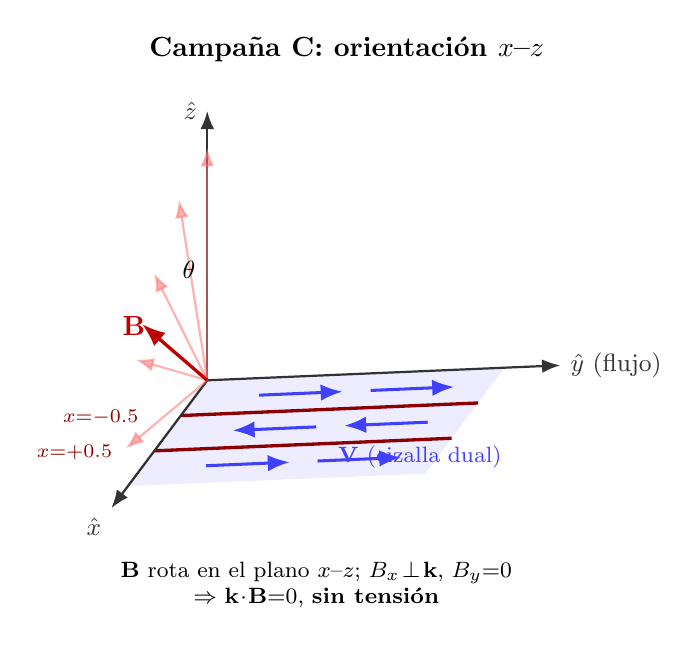
\begin{tikzpicture}[>=Latex,
  Bvec/.style={->,very thick,red!75!black},
  Bfan/.style={->,red!55,opacity=0.55,thick},
  flow/.style={->,blue!75,line width=1.1pt},
  ax/.style={->,thick,black!80}]
% proyeccion 3D->2D directa (px=x frente-izq, py=y derecha, pz=z arriba)
\newcommand{\PT}[3]{({(#1)*(-0.42)+(#2)*(1.18)+(#3)*(0)},{(#1)*(-0.56)+(#2)*(0.05)+(#3)*(1.18)})}
\def\Dx{2.4}\def\Dy{3.2}\def\ia{0.8}\def\ib{1.6}\def\L{2.5}

% plano de simulacion (grande)
\fill[blue!7] \PT{0}{0}{0} -- \PT{0}{\Dy}{0} -- \PT{\Dx}{\Dy}{0} -- \PT{\Dx}{0}{0} -- cycle;
\draw[very thick,red!55!black] \PT{\ia}{0}{0} -- \PT{\ia}{\Dy}{0};
\draw[very thick,red!55!black] \PT{\ib}{0}{0} -- \PT{\ib}{\Dy}{0};
\node[font=\scriptsize,red!55!black,anchor=east] at \PT{\ia}{-0.35}{0} {$x{=}{-}0.5$};
\node[font=\scriptsize,red!55!black,anchor=east] at \PT{\ib}{-0.35}{0} {$x{=}{+}0.5$};

% flujo dual: trasera +y, media -y, frontal +y
\foreach \yy in {0.7,1.9}{\draw[flow] \PT{0.4}{\yy}{0} -- \PT{0.4}{\yy+0.9}{0};}
\foreach \yy in {1.6,2.8}{\draw[flow] \PT{1.2}{\yy}{0} -- \PT{1.2}{\yy-0.9}{0};}
\foreach \yy in {0.7,1.9}{\draw[flow] \PT{2.0}{\yy}{0} -- \PT{2.0}{\yy+0.9}{0};}
\node[blue!75,font=\footnotesize] at \PT{2.0}{3.0}{0} {$\mathbf V$ (cizalla dual)};

% ejes
\draw[ax] \PT{0}{0}{0} -- \PT{2.9}{0}{0} node[below left,font=\small] {$\hat x$};
\draw[ax] \PT{0}{0}{0} -- \PT{0}{3.8}{0} node[right,font=\small] {$\hat y$ (flujo)};
\draw[ax] \PT{0}{0}{0} -- \PT{0}{0}{2.9} node[left,font=\small] {$\hat z$};

% campo C: abanico en plano x-z (rota de z hacia x)
\foreach \t in {0,20,40,60,80}{
  \draw[Bfan] \PT{0}{0}{0} -- \PT{\L*sin(\t)}{0}{\L*cos(\t)};
}
\draw[Bvec] \PT{0}{0}{0} -- \PT{\L*sin(52)}{0}{\L*cos(52)};
\node[red!75!black] at \PT{\L*sin(52)+0.25}{0}{\L*cos(52)+0.1} {$\mathbf B$};
\node[font=\small] at \PT{0.55}{0}{1.45} {$\theta$};
\node[font=\bfseries] at \PT{0}{1.5}{3.5} {Campaña C: orientación $x$--$z$};
\node[font=\footnotesize,align=center] at \PT{1.2}{1.6}{-1.7}
  {$\mathbf B$ rota en el plano $x$--$z$; $B_x\!\perp\!\mathbf k$, $B_y{=}0$\\ $\Rightarrow$ $\mathbf k\!\cdot\!\mathbf B{=}0$, \textbf{sin tensión}};
\end{tikzpicture}
\end{document}
